\subsection{Anti-Serialization}
In this section we will describe a set of transformation rules known as Anti-Serializations. In \cref{fig:trivial-example} all items made according to the three recipes in \cref{fig:toy-recipes} will have to pass through modules, which do not work on them. We would like to minimize this as to reduce the total length that each item must be transported, in addition to combating bottlenecks on the line. Thus it would be beneficial if items could bypass modules that do not work on them. We get around this by branching out production on more lines, where items only go through modules that work on them. 

\subsubsection{$AS_0$: Branch Between Common Modules}
We start by defining the most common type of anti-serialization with the $AS_0$ transformation rule given in \cref{def:as0}. Informally the rule states that if we have a set of modules $B_{r,s,e}$, which works the recipe $r \in R$ exclusivly, lying between the modules $s$ and $e$ on $\Gamma_0$ then we may branch out all modules in $B_{r,s,e}$ to form a new line. This new line is connected to $\Gamma_0$ at $s$ and $e$. We will explain this more in depth, by going over the sets brough up in the rule. 

\begin{definition}[htb]
\runatt{AS}{0}
    \infrule
        {0 < |B_{r,s,e}| \land  s <_k e}
        {(R,M,\Gamma, \Gamma_0, AW, Start, End) \rightarrow_{AS}
        (R,M,\Gamma', \Gamma_0', AW, Start', End') } \\
        Where: \\
        $r \in R$ \\
		$s,e \in K_{\Gamma_0,r}$\\		
		$\Gamma_0' = (Pre_s \cup \{s\}  \cup A_{r,s,e} \cup \{e\} \cup Pos_e, \prec)$ \\     
        $\Gamma' = (\Gamma \setminus \{\Gamma_0\}) \cup \{\Gamma_0'\} \cup B_{r,s,e} $ \\
		$Start' = Start \cup \{(B_{r,s,e}, s)\}$ \\
		$End' = End \cup \{(B_{r,s,e}, e)\}$

\caption{Formal definition of the $AS_0$ transformation rule}
\label{def:as0}
\end{definition}

We initially define a special set on $r$, $\bar{r}$, which contains all types of work which are not unique to $r$:
\[\bar{r} = \bigcup_{r' \in R}r', \texttt{ if } r' \neq r\]

Next we define, what we refer to as common modules. These are modules in $\Gamma_0$, which $r$ needs to use along with at least some other recipe. These are important to identify, as they may not be branched out, as that would make them inaccessible to the other recipes than $r$.  Given $r$ and $\Gamma_0$ we define the set of common modules $K_{\Gamma_0,r}$ as follows:

\[K_{\Gamma_0 ,r} = \{m | m \in \Gamma_0  \land \exists \rho \in AW(m),\, \{\rho\} \subseteq r \land \{\rho\} \subseteq \bar{r} \land r \in R\}\]

From this set we can then define $\alpha_{\Gamma_0 ,r}$, which is the set of modules in $\Gamma_0$ which are not used by $r$: 

\[\alpha_{\Gamma_0 ,r}  = \{m |m \in \Gamma_0 \land \forall \rho \in AW(m),\, \{\rho\} \nsubseteq r \land r \in R\}\]

Along with $\beta_{\Gamma_0 ,r}$, which is the set of modules in $\Gamma_0$ used only by $r$:

\[\beta_{\Gamma_0 ,r}  = \{m  | m \in \Gamma_0 \land \forall \rho \in AW(m),\, \{\rho\} \subseteq r \land \{\rho\} \nsubseteq \bar{r} \land r \in R\}\]

Next we define the binary relation relation $<_K$ as:
\[a <_K b = \left\{\begin{matrix}
tt \texttt{ if } a,b,c \in K_{\Gamma_0 ,r} \land a \prec b \land \lnot (a \prec c \land c \prec b) \\ \texttt{else } ff
\end{matrix}\right.\]

We also define a total order of all modules in between two modules, $s$ and $e$, in some line $\gamma \in \Gamma$:

\[M_{s,e} = (\{m | m \in \gamma \land \gamma \in \Gamma \land s \prec m \land m \prec e\}, \prec)\]

We can now define the total order of all modules appearing between $s$ and $e$, which are not used to work $r$, $A_{r,s,e}$ as follows: 

\[A_{r,s,e} = (\{m |m \in M_{s,e} \land m \in \alpha\}, \prec)\]

Similarly we can define the total order $B_{r,s,e}$, which contains all modules that appear between $s$ and $e$ which work exclusivly on $r$

\[B_{r,s,e} = (\{m |m \in M_{s,e} \land m \in \beta\}, \prec)\]

We define $Pre_{s}$ which is the set of all modules that come before a module $s$ in line $\gamma \in \Gamma$:
\[Pre_{s} = (\{m | m \in \gamma \land \gamma \in \Gamma \land m \prec s\}, \prec)\]

And lastly we define $Pos_{e}$ which is the set of all modules that come after a module $e$  in line $\gamma \in \Gamma$:
\[Pos_{e} = (\{m | m \in \gamma \land \gamma \in \Gamma \land e \prec  m \}, \prec)\]

Having defined these sets the rule in \cref{def:as0}, shows that in the case where $|B_{r,s,e}| > 0 \land s <_K e$ then we may update $\Gamma$ with two new lines, including an update of $\Gamma_0$ that describes a branch out from $\Gamma_0'$, which exclusivly works upon $r$ before rejoining with the old line.   

While this rule is formally sound it can be difficult to read. As such we have tried to illustrate the transformation from configuration to configuration visually in \cref{fig:as0}. This visualization uses a homemade notation. Square boxes refer to individual modules. Boxes with rounded corners are total orders of sets of modules. A graphical line of boxes flowing from left to right is a line in $\Gamma$ ordered as shown. If a module $s$ and a line $\gamma$ are connected by a vertical upward going edge, then $Start$ contains the ordered pair $(\gamma ,s)$. At the same time, if the edge goes downwards from a line $\gamma$ to a module $e$, then $End$ contains the ordered pair $(\gamma ,e)$.

%A box with rounded corners containing "..." means that here is a total order of one or more modules, but we do not care what they contain.

\begin{figure}[H]
\centering
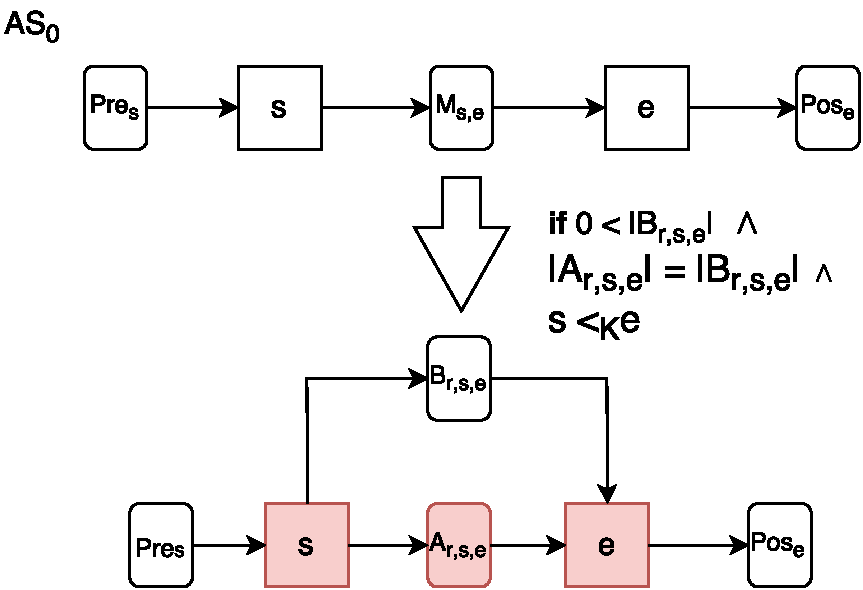
\includegraphics[width=\textwidth]{as0.pdf}
\caption{A visual representation of the $AS_0$ transformation rule}
\label{fig:as0}
\end{figure}

For the rest of this section, we will now use these visualization for explaining our transformation rules, instead of setting up transition rules. If any new derived sets are shown in a new transformation rule, we will describe them as well.  

In the rest of this sub-section we will describe two special cases known as $AS_1$, branch in, and $AS_2$,  branch out. 

\subsubsection{$AS_1$: Branch In}\label{sssec:bi}
It may be that we have modules that precede the first module of $K_{\Gamma_0 ,r}$ that we would like to branch out, but can't with the rule described in \cref{def:as0}, as it requires two distinct $K_{\Gamma_0 ,r}$ modules. So for this we describe the transformation rule $AS_1$, which can be seen in \cref{fig:as1}.

\begin{figure}[H]
	\centering
	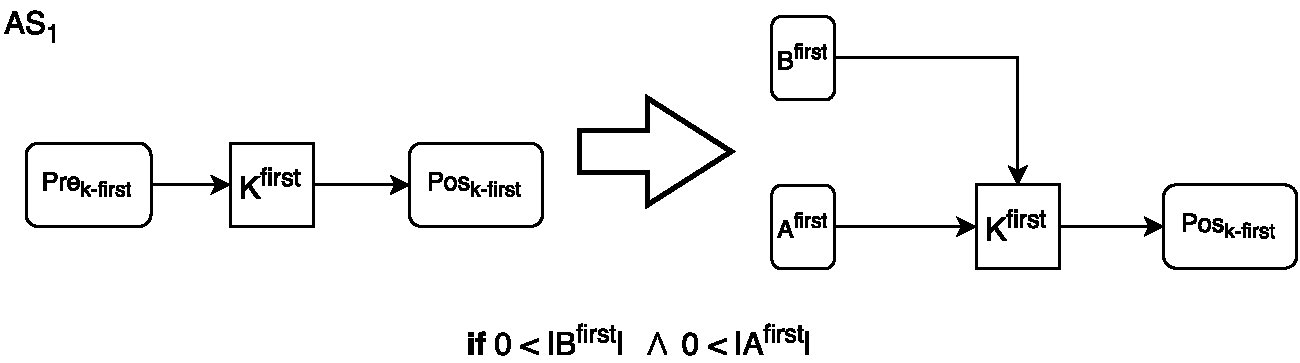
\includegraphics[width=\textwidth]{as1.pdf}
	\caption{A visual representation of the $AS_1$ transformation rule. This is used for the case where we which to branch out modules prior to the first element of $K_{\Gamma_0 ,r}$}
	\label{fig:as1}
\end{figure}


 We define the first module in $K_{\Gamma_0 ,r}$ as:

\[K_{\Gamma_0 ,r}^{first} = m \texttt{ where } \forall m' \in K_{\Gamma_0 ,r} \land m \neq m',\, m \prec m' \] 

Similarly for the $AS_0$ transformation rule, we define two total orderings. $A_{\Gamma_0 ,r}^{first}$ that describes all modules before $K_{\Gamma_0 ,r}^{first}$ on which $r$ does not perform any work. And $B_{\Gamma_0 ,r}^{first}$ which describes all modules before $K_{\Gamma_0 ,r}^{first}$ on which $r$ exclusively works.

\[ A_{\Gamma_0 ,r}^{first} = (\{m | m \in \alpha_{\gamma ,r}  \land m \in Pre_{K_{\Gamma_0 ,r}^{first}} \}, \prec) \]

\[ B_{\Gamma_0 ,r}^{first} = (\{m | m \in \beta_{\gamma ,r}  \land m \in Pre_{K_{\Gamma_0 ,r}^{first}} \}, \prec) \]

We also again use the $Pre_s$ and $Pos_e$ sets here, but used on $K_{\Gamma_0 ,r}^{first}$ instead of $s$ and $e$.
  

\subsubsection{$AS_2$: Branch Out}
Similarly to $AS_1$ we have the case where the last element in $K_{\gamma ,r}$, is proceeded by a set of modules that we would like to branch out. For this we describe the transformation rule $AS_2$, which can be seen in \cref{fig:as2}.

\begin{figure}[H]
	\centering
	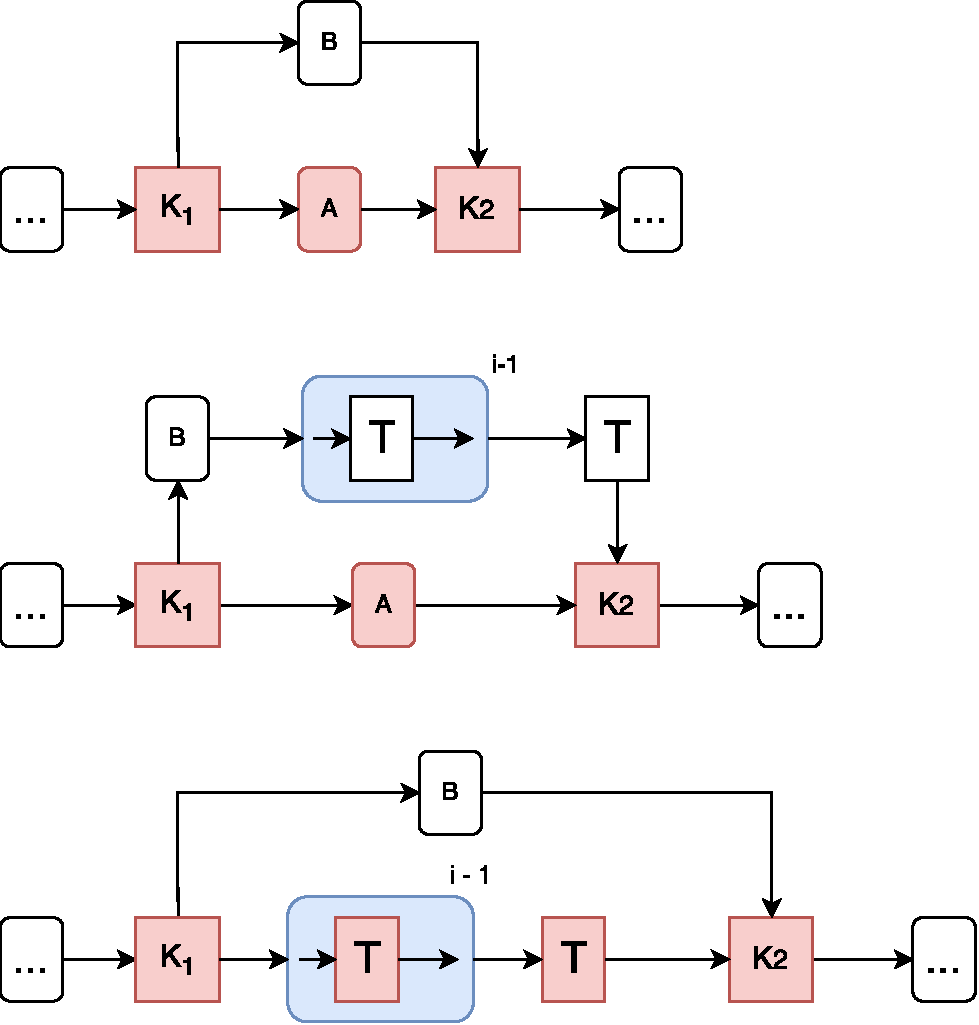
\includegraphics[width=\textwidth]{as2.pdf}
	\caption{A visual representation of the $AS_2$ transformation rule. This is used for the case where we which to branch out modules proceeding the last element of $K_{\Gamma_0 ,r}$}
	\label{fig:as2}
\end{figure}


We define the last module in $K_{\Gamma_0 ,r}$ as:

\[K_{\Gamma_0 ,r}^{last} = m \texttt{ where } \forall m' \in K_{\Gamma_0 ,r} \land m \neq m',\, m' \prec m \] 


Again we also define two total orders. $A_{\Gamma_0 ,r}^{last}$ that describes all modules after $K_{\Gamma_0 ,r}^{last}$ on which $r$ does not perform any work. And $B_{\Gamma_0 ,r}^{last}$ which describes all modules after $K_{\Gamma_0 ,r}^{last}$ on which $r$ exclusively works.


\[ A_{\Gamma_0 ,r}^{last} = \{m | m \in \alpha_{\gamma ,r}  \land m \in Pos_{K_{\Gamma_0 ,r}^{last}} \} \]

\[B_{\Gamma_0 ,r}^{last} = \{m | m \in \beta_{\gamma ,r}  \land m \in Pos_{K_{\Gamma_0 ,r}^{last}} \}\]



%\subsubsection{Restricting branches}
%For the previous transformation rules, we have imagined that no other branch has been made from our line to any side. Yet, this will not always be the case. To be flexible enough to produce configurations with high throughput, we need to handle this. We go more in depth with how to enforce some general physical rules in \cref{ssec:conflicts}, but here we will tackle one unique to anti-serialization.

%On the top part of \cref{fig:shadowexample}, we see that we have already made a branch from $s1$ to $e1$, which results in the modules on the old being shadowed. Being shadowed means that if we remove the module and just reconnect the old line as usual, then the branch becomes too long to connect back to its old line. The line needs to connect back to its designated point on the old line as the module located here is a common module. It performs work on the recipe $r$ otherwise worked on by the new line and should therefore not be bypassed.  To get around this we, as shown in \cref{fig:shadowexample}, alter our anti-serialization transformation in this case to replace a shadowed module with a transport module, as not to skew the two previous lines away from each other. The example shows this done for a single module, but it may be done regardless of the amount of shadowed modules which we remove.

%We may however not do this if the shadowed module is also a module where a branch either connects from or to. This means that the module is common and is used by the branch. Removing it would keep us from producing that branch's specific recipe. Therefore we never allow for these modules to be removed, even if this means that we can not perform certain anti-serializations.

%\begin{figure}[H]
%\centering
%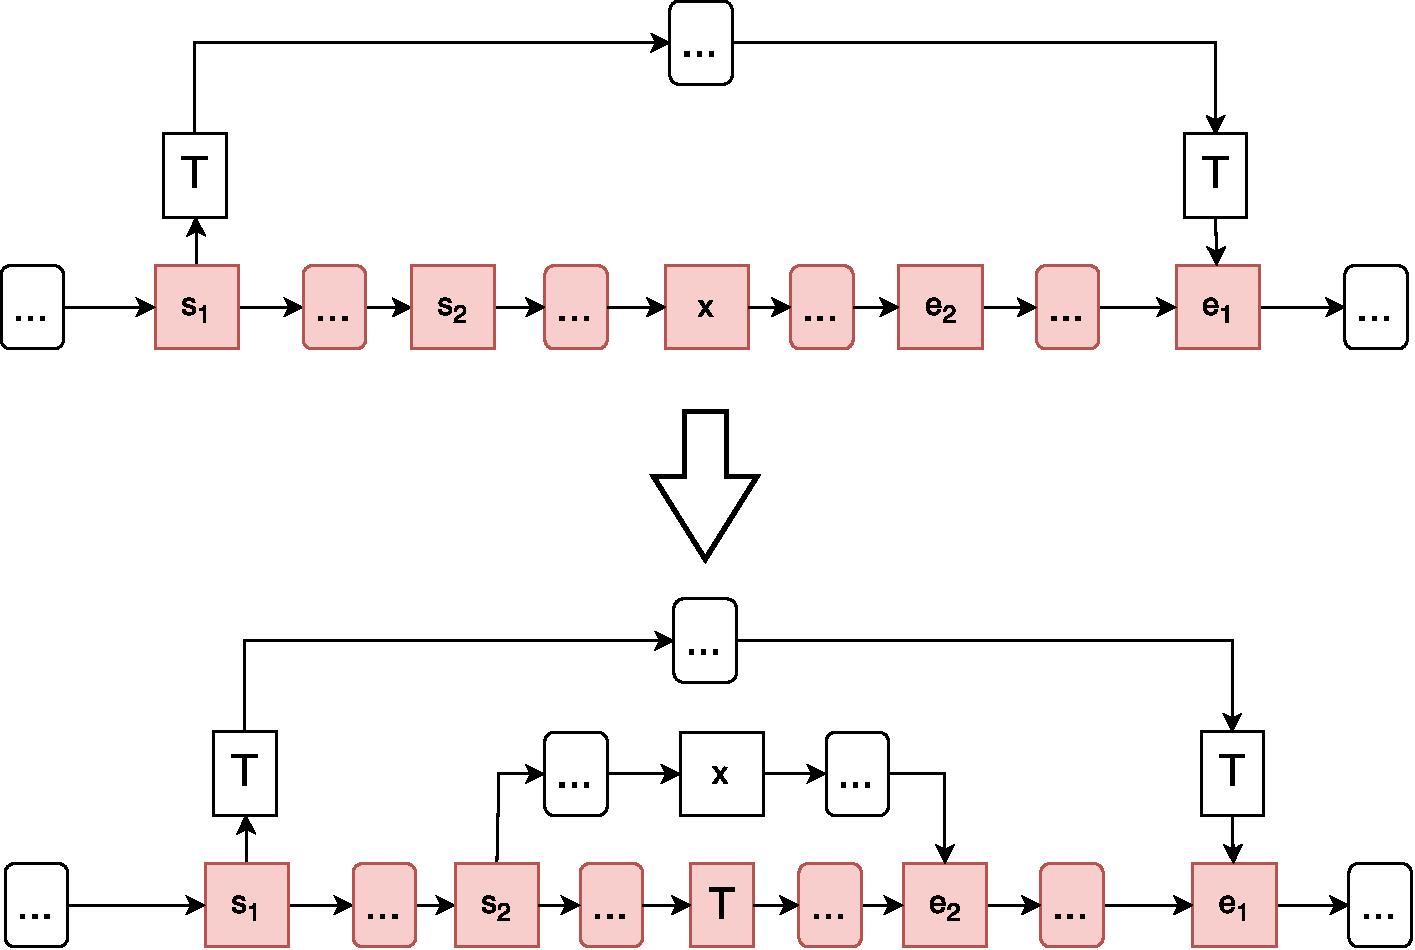
\includegraphics[width=\textwidth]{as5.pdf}
%\caption{Transformation that handles the case where an %anti-serialization removes a shadowed module}
%\label{fig:shadowexample}
%\end{figure}


%Now imagine the situation in \cref{fig:asbase}. Here we have specific $s$ and $e$ modules chosen on a line $\gamma$ and we have chosen to branch out a specific recipe $r$. Between the two modules we may have $M_{s,e}$ placed. From this we can calculate $A_{s,e}$ and $B_{s,e}$ as described before. If $B_{s,e} = \emptyset$ then we may branch out some modules only used to work on $r$. 

%If $|A_{s,e}| = |B_{s,e}| + 2$ , then we can branch out as shown in the top of \cref{fig:astrans}. Here we simply remove $|B_{s,e}|$ from the rest of $M_{s,e}$ leaving us with in its place $A_{s,e}$. The module $s$ is then connected upwards to the first element of $|B_{s,e}|$. The last element of $|B_{s,e}|$ is then connected to $e$. This transformation also entails that all of  $|B_{s,e}|$ is removed from $\gamma$ and that a new line containing $|B_{s,e}|$ is added to $\Gamma$. For each of the transformations presented in this subsection we alter $\gamma$ and add to $\Gamma$ the new branch which is created.  Notice that the modules beneath the new line are marked as red. This means that the shadow variable in the module tuples on the old line have been set to true. This is used in order to handle transformation conflicts as described later in \cref{ssec:tc}.

%In the middle of \cref{fig:astrans} we describe the case where $A_{s,e}| > |B_{s,e}| + 2$. The difference between the cardinality of these two sets is called i.  In this case we can not physically connect the last element of $|B_{s,e}|$ downwards to $e$. We get around this issue by appending the new line with i new transport modules. These are modules which can not perform any work and are only used to transport recipes. The last of these transporters is then connected downwards to $e$. The new line added to $\Gamma$ consists of the modules in $|B_{s,e}|$ ordered behind the new transport modules as depicted in the figure. 

%The last case, shown in the bottom of \cref{fig:astrans} is similar to the previous one, but instead $A_{s,e}| < |B_{s,e}| + 2$. In this case we append the original line with transporters instead. This requires an update of $\gamma$ to include these new transporters, while the new line added to $\Gamma$ is again just $|B_{s,e}|$. 

%\begin{figure}[H]
%\centering
%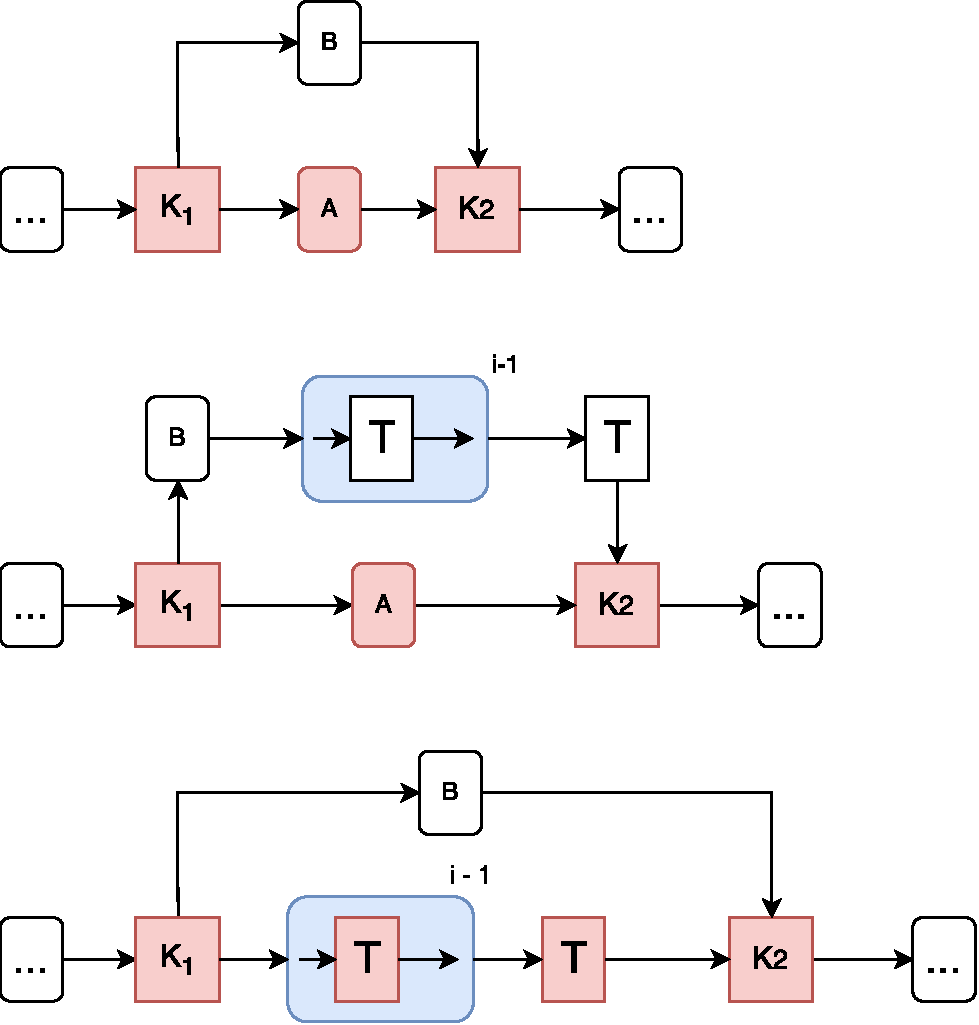
\includegraphics[width=\textwidth]{as2.pdf}
%\caption{3 different configurations to which we may go from %\cref{fig:asbase}. Top: Case when $A_{s,e}| = |B_{s,e}| + 2$. Middle: Case when $A_{s,e}| > |B_{s,e}| + 2$. Bottom: Case when $A_{s,e}| < |B_{s,e}| + 2$ }
%\label{fig:astrans}
%\end{figure}
